\chapter{The monolithic VMS engine}
\label{ch:c1}

\emph{Module: \file{01\_monolithic\_vms/}. The oracle. One coupled saddle
solve per step; the lid-driven cavity vs Ghia.}

\section{Galerkin weak form}
Test momentum with $w$ and continuity with $q$. Integrate the viscous and
pressure terms by parts and drop the do-nothing surface terms
(\file{ns\_bricks.py:16--21}):
\begin{align}
\intv w\cdot\partial_t u + \intv w\cdot(u\cdot\grad)u
  + \nu\intv \grad w:\grad u - \intv (\grad\cdot w)\,p &= \intv w\cdot f,\\
\intv q\,(\grad\cdot u) &= 0.
\end{align}

\section{Residual-based VMS: the fine scale $u' = -\tauM R_M$}
VMS splits $u=\uh+u'$ into a resolved (coarse) scale $\uh$ and an
unresolved (fine) scale $u'$, modeled algebraically as $u'=-\tauM
R_M(\uh,\ph)$, where $R_M$ is the momentum strong residual. Substituting
$u'$ back into the weak form and integrating the fine-scale terms produces
three stabilization contributions (\file{ns\_bricks.py:23--27},
\file{44--51}):
\begin{itemize}
\item \textbf{SUPG} (streamline-upwind on the momentum test):
  $\tauM\,(a\cdot\grad w)\cdot R_M$;
\item \textbf{PSPG} (pressure-stabilizing, on the continuity test):
  $\tauM\,(\grad q)\cdot R_M$ --- \emph{this is the term that makes
  equal-order work};
\item \textbf{grad-div / LSIC}: $\tauC\,(\grad\cdot w)(\grad\cdot u)$.
\end{itemize}

\section{The stabilization parameters}
The monolithic stepper uses the \textbf{metric-tensor} $\tau$ form
(\file{physics/vms.py:5--12}, \file{38--45}). On DiffSim's axis-aligned
octree cubes the element metric is diagonal, $G=(2/h)^2 I$, so
\begin{equation}
\tauM = \Big[\Big(\tfrac{2b_0}{\Delta t}\Big)^2 + \tfrac{4|u|^2}{h^2}
  + C_I\,\nu^2\,\dim\,\big(\tfrac{2}{h}\big)^4\Big]^{-1/2},\quad C_I=36,
\qquad
\tauC = \frac{1}{\tauM\,\dim\,(2/h)^2}.
\end{equation}
The transient term $(2b_0/\Delta t)^2$ is present when \code{timestab=True}
(dropped for steady/order studies). The device functions are
\code{tau_m_metric} / \code{tau_c_metric} (\file{physics/vms.py:60--74}).

\begin{keybox}\textbf{Key idea.} The projection engine instead uses the
\emph{h-based} $\tau$ form, whose defaults reproduce the metric form on
cubes \emph{by construction} (\file{physics/vms.py:13--19}). So the two
engines are comparable term-for-term on these meshes --- which is exactly
what makes the faithfulness comparison meaningful.\end{keybox}

\section{The saddle system $\saddle$}
After linearization, each node block is the full
$(\dim+1)\times(\dim+1)$ coupling written by the element kernel
\code{lin_ns_Ae} (\file{ns\_bricks.py:341--447}):
\begin{itemize}
\item \textbf{$F$} (velocity--velocity): mass $\sigma N_a N_b$ + convection
  $N_a(a\cdot\grad N_b + s(\grad\!\cdot a)N_b)$ + viscous
  $\nu\,\grad N_a\!:\!\grad N_b$ + SUPG $\tauM(a\cdot\grad N_a)R_{M,b}$ +
  grad-div $\tauC\,\partial_i N_a\,\partial_j N_b$.
\item \textbf{$G$} (velocity--pressure): $-\partial_i N_a\,N_b$ plus the
  SUPG pressure coupling $\tauM(a\cdot\grad N_a)\,\partial_i N_b$.
\item \textbf{$D$} (continuity--velocity): $N_a\,\partial_i N_b$ plus the
  PSPG velocity coupling $\tauM\,\partial_i N_a\,R_{M,b}$.
\item \textbf{$C$} (the \emph{PSPG C-block}): $\tauM\,\grad N_a\cdot\grad
  N_b$. This nonzero pressure--pressure block is exactly what stabilizes
  the equal-order pair (\file{ns\_bricks.py:442--444}).
\end{itemize}

\section{Time integration and convection linearization}
The transient term uses backward differencing (BDF1 bootstrap $\to$ BDF2).
Per step $\sigma=b_0/\Delta t$ enters the mass term and $\tauM$; the
history $-(b_1 u^n+b_2 u^{n-1})/\Delta t$ becomes part of the linearized
strong residual (\file{linearized.py:181--226}). The nonlinear convection
$(u\cdot\grad)u$ is handled by an \textbf{advecting field} $a$ precomputed
at Gauss points --- a fine-scale-corrected BDF \emph{extrapolation}
(Picard/Oseen, default) or Newton (adds the cross-term block). The
convection uses the \textbf{skew-symmetric} form
$a\cdot\grad u + s(\grad\!\cdot a)u$ with $s=\tfrac12$ (energy-stable).

\section{Code walkthrough}
\code{assemble_linear_ns(dm, aq, div_aq, fq, nu, sigma, ...)}
(\file{ns\_bricks.py:507--562}) builds the constrained node-major saddle
matrix $A$ and RHS $b$; it launches \code{lin_ns_Ae} (matrix) and
\code{lin_ns_be} (RHS) per element bin, then constrains with
$T_{\text{vec}}=T\otimes I_{\dim+1}$.
\code{LinearizedMonolithicStepper.step()} (\file{linearized.py:181--245})
orchestrates one step: BDF coefficients, build $a$, assemble, apply strong
velocity Dirichlet rows + a single pressure pin, solve, rotate history.

\section{Verification: the lid-driven cavity vs Ghia}
The module marches the \emph{same mesh} with \emph{both} engines and
compares the $x=0.5$ centerline $u(y)$ against Ghia, Ghia \& Shin (1982),
Table~I. On a level-4 ($16\times16$) mesh at $\Rey=100$:
\begin{center}
\begin{tabular}{@{}lccc@{}}
\toprule
station $y$ & projection $u$ & monolithic $u$ & Ghia $u$\\
\midrule
0.9766 & $+$\LdcProjLid & $+$\LdcMonoLid & $+$\LdcGhiaLid\\
\bottomrule
\end{tabular}
\end{center}
\[
\max|\text{proj}-\text{mono}| = \LdcProjMono,\quad
\max|\text{proj}-\text{Ghia}| = \LdcProjGhia,\quad
\max|\text{mono}-\text{Ghia}| = \LdcMonoGhia.
\]
The coarse level-4 mesh cannot resolve Ghia's $129^2$ table to the third
digit --- that is expected. The decisive checks are (a) the projection
tracks the monolithic on the \emph{same} mesh and (b) both track Ghia
within the coarse-mesh tolerance.

\begin{figure}[h]\centering
\IfFileExists{figures/c1_centerline.png}
  {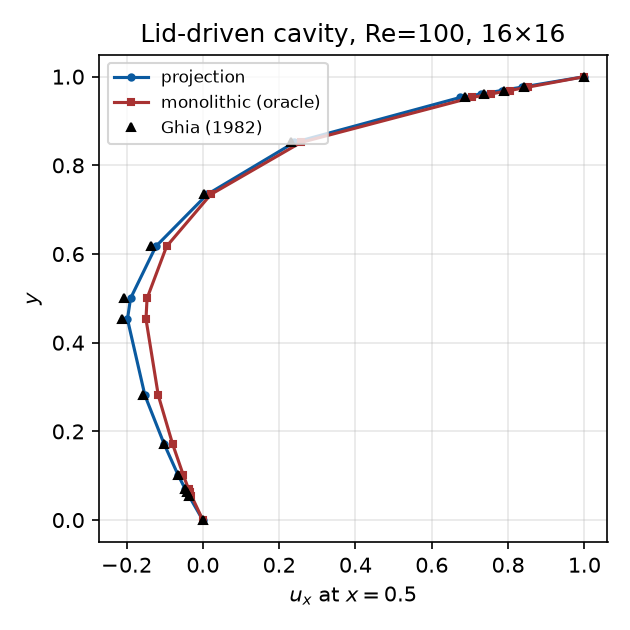
\includegraphics[width=0.5\textwidth]{figures/c1_centerline.png}}{}
\caption{Lid-driven cavity centerline $u_x(y)$ at $x=0.5$: the projection
and monolithic engines vs the Ghia (1982) table, on a level-4 mesh.
Regenerated by \file{01\_monolithic\_vms/gen\_figures.py}.}
\end{figure}

\begin{keybox}\textbf{Key idea.} The pointwise $\|\grad\!\cdot u\|$ of the
equal-order VMS scheme is \emph{not} driven to zero
(\LdcDivMono{} here for the monolithic). The scheme controls the
\emph{weak} divergence; a finite, bounded $\|\grad\!\cdot u\|$ is correct,
and it is the wrong steady-state gate.\end{keybox}

\begin{runbox}\textbf{Run it.} \code{python run.py} in
\file{01\_monolithic\_vms/} marches both engines and prints the centerline
table. \code{--level 5} tightens toward Ghia (slower); \code{--Re 400}
needs more steps.\end{runbox}

\question The viscous term $-\nu\,\Delta \uh$ in the linearized residual is
identically zero at $P_1$ but required at $P_2$. Why? (Hint: second
derivatives of $Q1$ shape functions.)

\question Force \code{--solver cudss} on this small cavity. Does it help or
hurt? Relate your answer to whether the saddle is definite.
